% Figure: the orbit coordinate and the canonical gauge. Referenced from §6, before
% prop:canonical-gauge. Pure TikZ. Paper I's fig-orbit-gauge with this article's letters (the
% scale t, the ratio lambda, the gauge chi). A concrete gauge for the drawing: chi(t) = t^2, so
% S_lambda 1 = sqrt(lambda) on the raw axis; panel (a) unit 3cm, panel (b) unit 1.5cm.

\begin{figure}[!htb]
\centering
\begin{tikzpicture}[every node/.style={font=\small}, line cap=round, >=stealth]

% ---------- panel (a): the scale axis as given ----------
\begin{scope}[yshift=0cm]
  \node[anchor=west] at (-0.3,1.7) {(a) the scale axis as given: the orbit of $1$ under $S_\lambda$};
  \draw[->] (0,0) -- (8.0,0) node[right] {$t$};
  \draw (0,0.07) -- (0,-0.07); \node[below] at (0,-0.05) {$0$};
  \foreach \p/\l in {2.12/$S_{1/2}1$, 3/$1$, 4.24/$S_{2}1$, 6/$S_{4}1$} {
    \draw (\p,0.07) -- (\p,-0.07); \node[below] at (\p,-0.05) {\l};
  }
  \fill (3,0) circle (1.6pt);
  \draw[->,dashed] (3,0.15) to[bend left=35] node[above] {$S_2$} (4.24,0.15);
  \draw[->,dashed] (4.24,0.15) to[bend left=35] node[above] {$S_2$} (6,0.15);
  \draw[->,dashed] (3,0.15) to[bend right=35] node[above] {$S_{1/2}$} (2.12,0.15);
  \node[anchor=west] at (0,-0.75) {equal ratios of $\lambda$, unequal steps on the axis};
\end{scope}

% ---------- panel (b): the same axis in the canonical gauge ----------
\begin{scope}[yshift=-3.6cm]
  \node[anchor=west] at (-0.3,1.7) {(b) the canonical gauge $\tilde t = \chi(t)$: the same action is multiplication};
  \draw[->] (0,0) -- (8.0,0) node[right] {$\tilde t$};
  \draw (0,0.07) -- (0,-0.07); \node[below] at (0,-0.05) {$0$};
  \foreach \p/\l in {0.75/$\tfrac12$, 1.5/$1$, 3/$2$, 6/$4$} {
    \draw (\p,0.07) -- (\p,-0.07); \node[below] at (\p,-0.05) {\l};
  }
  \fill (1.5,0) circle (1.6pt);
  \draw[->,dashed] (1.5,0.15) to[bend left=35] node[above] {$\times 2$} (3,0.15);
  \draw[->,dashed] (3,0.15) to[bend left=35] node[above] {$\times 2$} (6,0.15);
  \draw[->,dashed] (1.5,0.15) to[bend right=35] node[above] {$\times \tfrac12$} (0.75,0.15);
  \node[anchor=west] at (0,-0.75) {$\chi(S_\lambda t) = \lambda\,\chi(t)$: equal ratios of $\lambda$, equal ratios on the axis};
\end{scope}

\end{tikzpicture}
\caption{The orbit coordinate. (a)~On the scale axis as the family presents it, the action
$S_\lambda$ of (A8) is some increasing bijection. The orbit of the point $1$,
$\lambda \mapsto S_\lambda 1$, is continuous, strictly increasing and has no fixed point, so
it sweeps all of $t > 0$ (Lemma~\ref{lem:action-rigidity},
Proposition~\ref{prop:canonical-gauge}). The given scale labels need not preserve dilation
ratios, and the canonical coordinate does: equal ratios of $\lambda$ are unequal steps on the
axis. (b)~Labelling each point by the $\lambda$ that reaches it, $\tilde t = \chi(t)$, the
same action becomes multiplication by $\lambda$: the canonical gauge. In this gauge every
accumulated exponent is a dilate of one function, $G(t,\omega) = F(\tilde t\,\omega)$.}
\label{fig:orbit-gauge}
\end{figure}
